\chapter{Analysis and prediction of seiyuu popularity}

Popularity is an abstract criterion that must be defined as a numerical metric in order to be used for analysis and prediction. Since we are using MAL database and it has a social component, seems logic to use member\_favorites as a representation of popularity. We can also get popularity and score of anime from opinions of the same set of users.\\

In terms of distribution \textit{popularity} is highly unequal \---as we can observe in Fig.~\ref{fig:popularityDistribution}\--- having a lot of seiyuu which are no member favorites and only a few who are favorite of more than 10000 members. It's good to keep in mind that users can favorite multiple seiyuu.

\begin{figure}[!h]
	\begin{center}
	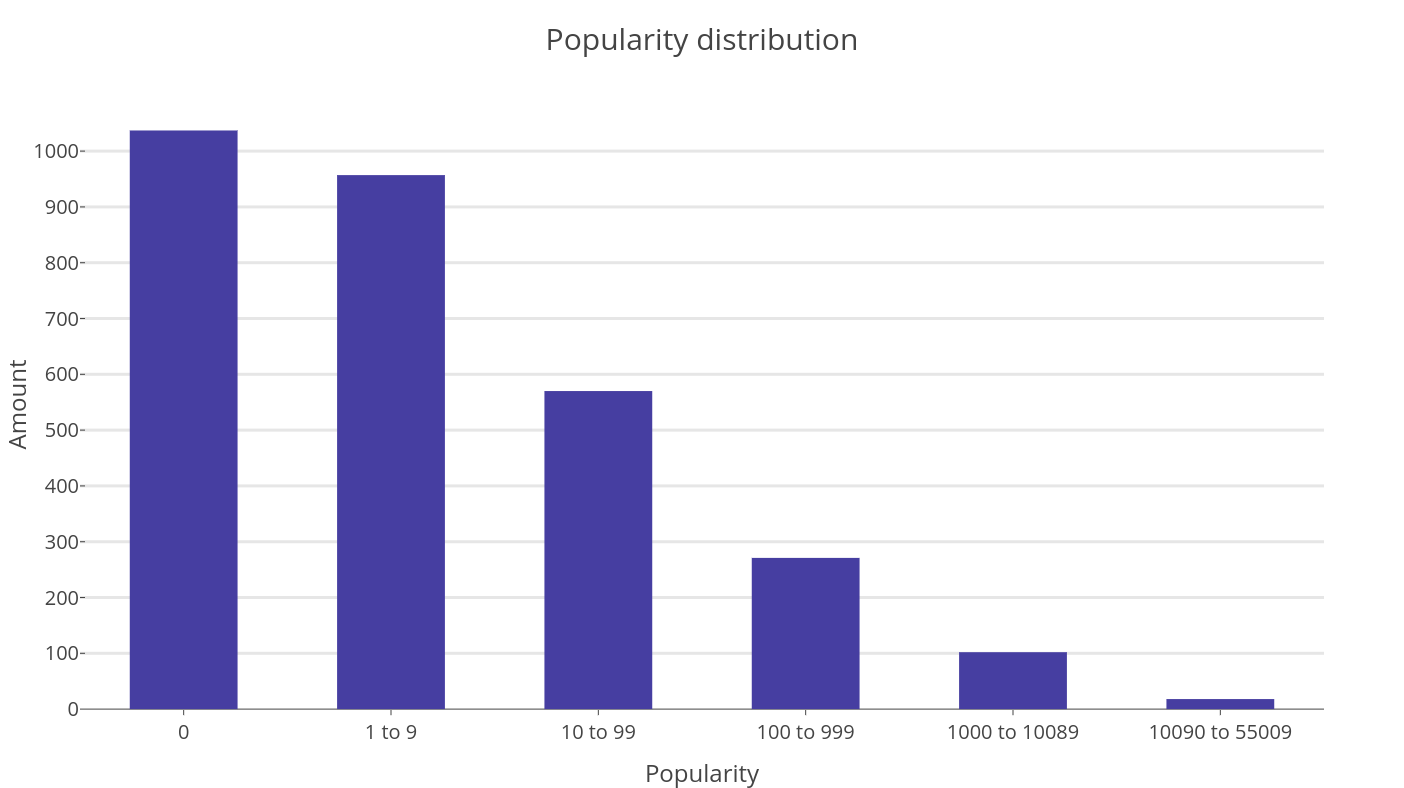
\includegraphics[width=\columnwidth]{graphics/popularityDistribution.png}
	\caption{Amount of seiyuu with that popularity, divided into groups for better visualization.}
	\label{fig:popularityDistribution}
	\end{center}
\end{figure}

\newpage

Some metrics about popularity:
\begin{itemize}
	\item Mean:    289.55
	\item Median:    2.0
	\item Max:    55018
	\item Min:    0 
	\item 1037 values equal to zero
	\item Only 120 values bigger than 1000
\end{itemize}

\begin{table}[!h]
	\begin{center}
	\caption{Top 10 popular seiyuu}
	\label{tab:top10Popularity}
	\begin{tabular}{|l|c|}
		\hline
		Name & Popularity \\ 
		\hline
		Kana Hanazawa & 56637 \\ 
		\hline
		Hiroshi Kamiya & 49685 \\ 
		\hline
		Mamoru Miyano & 43942 \\ 
		\hline
		Rie Kugimiya & 31668 \\ 
		\hline
		Jun Fukuyama & 26811 \\ 
		\hline
		Miyuki Sawashiro & 26501 \\ 
		\hline
		Tomokazu Sugita & 24449 \\ 
		\hline
		Daisuke Ono & 24080 \\ 
		\hline
		Saori Hayami & 18322 \\ 
		\hline
		Aya Hirano & 18094 \\ 
		\hline
	\end{tabular}
	\end{center}
\end{table}

\section{Correlation with only one feature}
As shown in Fig.~\ref{fig:pearsonCorr} our first approach to explaining popularity was using Pearson correlation. 
\textbf{TODO PONER UN GRAFO DE PEARSON CON CASI TODOS LOS PARAMETROS POSIBLES EN VEZ DE EL QUE ESTA AHORA}

\begin{figure}[!h]
	\begin{center}
	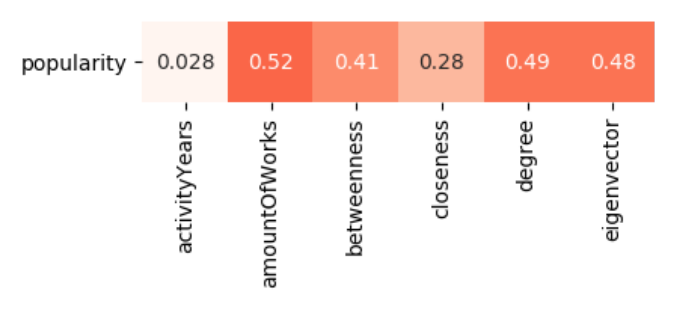
\includegraphics[width=\columnwidth]{graphics/10Works_correlation_Pearson.png}
	\caption{Pearson correlation between popularity and some features of nodes.}
	\label{fig:pearsonCorr}
	\end{center}
\end{figure}

A fairly big correlation can be seen between popularity and amount of works. Since this data is biased to more modern anime we thought of trying to correlate with more recent works only. But, how recent? Last 5, 10 or 20 years? Thus correlation between popularity and works from different data frames was analyzed, Fig.~\ref{fig:correlationPopRecentWorks}.

\begin{figure}[!h]
	\begin{center}
	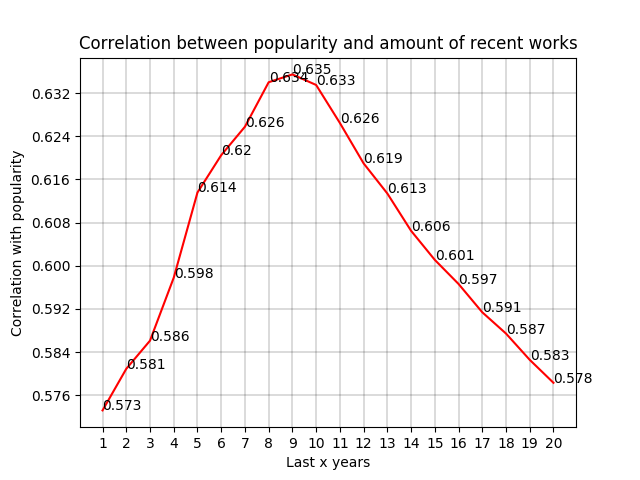
\includegraphics[width=\columnwidth]{graphics/correlationPopRecentWorks.png}
	\caption{Last \textit{X} years means works from 2018-\textit{X} to present.}
	\label{fig:correlationPopRecentWorks}
	\end{center}
\end{figure}

The best result was given by recent works from last 9 years. Therefore, this definition of recent works was used from there on.

\FloatBarrier
\subsection{Why last 9 years of works has more correlation?}
Graphics of some characteristics of works divided by years were made, trying to shed some light over why works from last 9 years were more "important". 

\begin{sidewaysfigure}
	\centering
	\begin{subfigure}{.55\columnwidth}
		\centering
		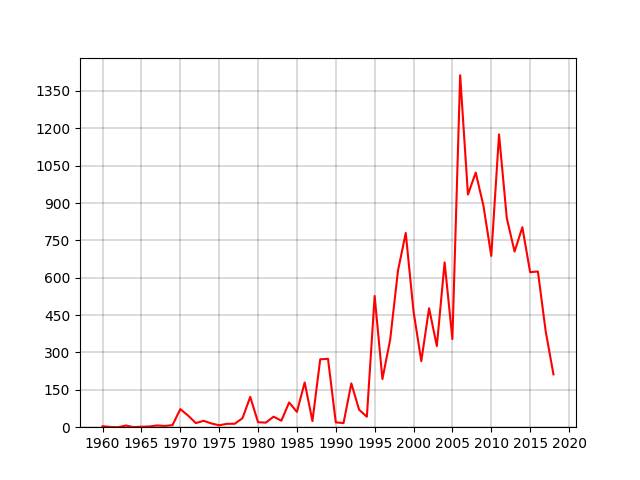
\includegraphics[width=\columnwidth]{graphics/avgFavorites.png}
		\caption{Average amount of favorites per year.}
		\label{fig:avgFavorites}
	\end{subfigure}%
	\begin{subfigure}{.55\columnwidth}
		\centering
		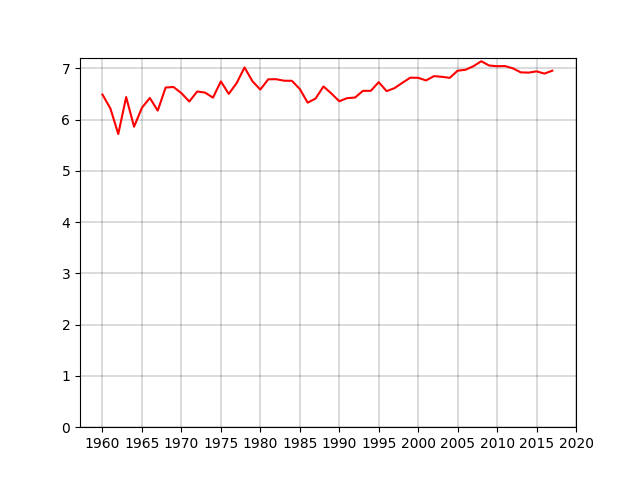
\includegraphics[width=\columnwidth]{graphics/avgScores.png}
		\caption{Average score per year.}
		\label{fig:avgScores}
	\end{subfigure}
	\begin{subfigure}{.55\columnwidth}
		\centering
		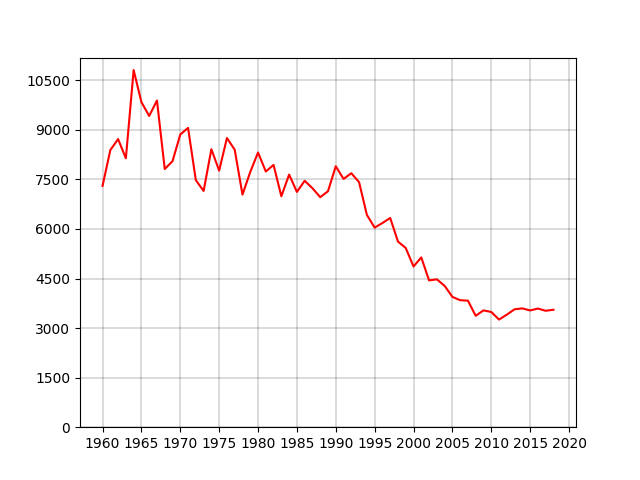
\includegraphics[width=\columnwidth]{graphics/avgPopularities.png}
		\caption{Average popularity per year.}
		\label{fig:avgPopularities}
	\end{subfigure}%
	\begin{subfigure}{.55\columnwidth}
		\centering
		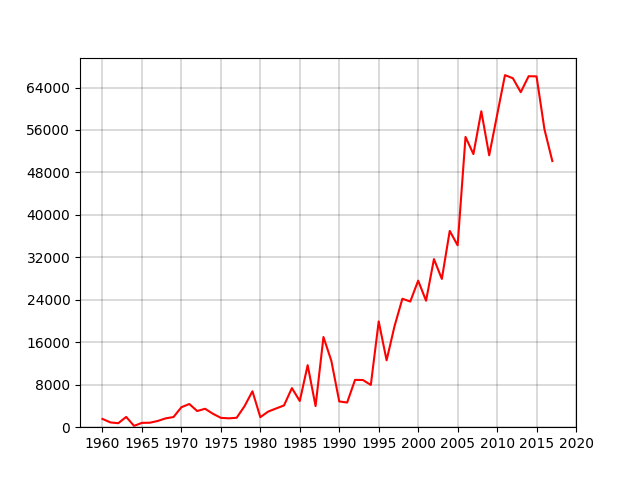
\includegraphics[width=\columnwidth]{graphics/avgMembers.png}
		\caption{Average amount of members per year.}
		\label{fig:avgMembers}
	\end{subfigure}
	\caption{Averages of some atributes of anime divide by year.}
	\label{fig:averages}
\end{sidewaysfigure}

Fig.~\ref{fig:avgFavorites} and ~\ref{fig:avgScores} shows an improvement in average of scores and favorites. 

Biggest peak of favorites is on 2005, this may have to do with the start of MAL (2006), see Fig.~\ref{fig:avgFavorites}. We suppose as users started to use MAL they favorite anime they liked from that year and only some of the old ones; from then on they used the website often and favorite new works as they began airing.

2018 was left out of Fig.~\ref{fig:avgScores} because, since 2018 is not finished yet, the average of scores was unusually small.

As Fig.~\ref{fig:avgPopularities} shows, popularity goes down in last years. But we need to consider that this metrics are from MAL and it could mean, for example, the parameter is in disuse; instead of representing how people feel about new anime.\\

We suppose the attribute "members" of an anime is taken from how many users have it on any of their lists. If that is correct Fig.~\ref{fig:avgMembers} tells us feature of adding anime in watched / watching / plan to watch lists is really used. As for our experience on the web and social media we can confirm this is the most used feature of MAL. So this makes it one of the best metrics to measure "public" as another sense of popularity of anime.\\

As we can see on Fig.~\ref{fig:amountOfWorksPerYear} anime industry is growing bigger each year, of course this is biased by the fact MAL will sure have every adaptation of last year but maybe not for anime from 1980.

\begin{figure}[!h]
	\begin{center}
	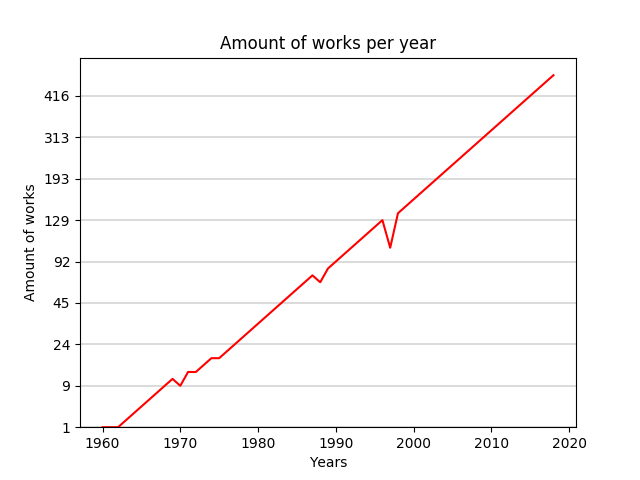
\includegraphics[width=\columnwidth]{graphics/worksPerYear_1960-2018.png}
	\caption{Amount of works divided by years which were aired for the first time.}
	\label{fig:amountOfWorksPerYear}
	\end{center}
\end{figure}

The majority of works are from 1990 to 2018 and half of them are distributed over the last 14 years (2014 to 2018) but as far as we can tell there isn’t anything particular over the last 9 years nor on year 2009. Judging by amount of favorites per year it appears that users have been more active in recent years so this could be one of the reasons.

\section{Correlation with multiple features}
For this section Scikit-learn, a free software machine learning Python library, was used. The node attributes were divided into categories, leaving four distinct types:

\begin{itemize}
	\item Personal data:
	\begin{itemize}
		\item Debut
		\item Gender
		\item Activity years (2018-debut)
	\end{itemize}
	\item Works data:
	\begin{itemize}
		\item Amount
		\item Top 5 genre
		\item Favorites
		\item Score
		\item Popularity
		\item Members
	\end{itemize}
	\item Recent works data:
	\begin{itemize}
		\item Same as works but for only last 9 years
	\end{itemize}	
	\item Graph data:
	\begin{itemize}
		\item Degree
		\item Betweenness centrality
		\item Closeness
	\end{itemize}
\end{itemize}

Fitting and prediction experiments were run for each category, each combination of 2, 3 and all of them together; using 80\% of seiyuu as train data and the rest as test. This was done for all following models:
\begin{itemize}
	\item DecisionTreeRegressor
	\item DecisionTreeClassifier
	\item LinearRegression
	\item KNeighborsClassifier
	\item LinearDiscriminantAnalysis
	\item GaussianNB
	\item SVM
\end{itemize}

We have to take into account popularity variance when trying to predict it since usual error metrics don't distinguish between small or big values. If we predict exactly a seiyuu that has \textgreater50000 popularity but we make "small" mistakes predicting seiyuu with \textless100 popularity then, is it a good prediction? and having into account more than $\frac{3}{4}$ of them have \textless100 popularity?

To compare prediction performance mean and median absolute error were used. Unfortunately since popularity variance is really high we observed good results in terms of absolute error but particular predictions were aloof. This is why we use r2\_score\footnote{\url{http://scikit-learn.org/stable/modules/model_evaluation.html#r2-score-the-coefficient-of-determination}} for accuracy comparation. 

\textbf{TODO SHOW TABLE WITH R2 SCORE RESULTS FOR EACH CATEGORY / MODEL AND GROUP OF CATEGORIES}\\
\textbf{TODO ADD SOME OF THE GRAPHICS ABOUT FEATURE IMPORTANCE FOR DTC (ONLY BEST ONES) AND EXPLAIN (FOR EACH SUBSECTION)}

\FloatBarrier
\subsection{Only one category}
\begin{table}[!hbt]
	\begin{center}
	\caption{Only one category R2 score results}
	\label{tab:oneCategory}
	\begin{tabular}{|l|c|c|c|c|}
		\hline
		Model / Data & Recent works & Personal & Graph & Work \\ 
		\hline
		DecisionTreeClassifier & 0.11 & -0.04 & 0.06 & -1.3 \\ 
		\hline
		DecisionTreeRegressor & 0.33 & -0.29 & -0.05 & 0.11 \\ 
		\hline
		GaussianNB & 0 & -4.7 & -0.03 & 0 \\ 
		\hline
		KNeighborsClassifier & 0.22 & -0.04 & 0.06 & -0.05 \\ 
		\hline
		LinearDiscriminantAnalysis & 0.47 & -0.04 & 0.32 & -1.04 \\ 
		\hline
		LinearRegression & 0.57 & 0 & 0.28 & 0.42 \\ 
		\hline
		SVM & -0.02 & -0.04 & -0.01 & -0.02 \\ 
		\hline
	\end{tabular}
	\end{center}
\end{table}

\FloatBarrier
\subsection{Groups of two categories}
\begin{table}[!hbt]
	\begin{center}
	\caption{Two categories R2 score results (R: recent works, P: personal, G: graph, W: work)}
	\label{tab:twoCategories}
	\begin{tabular}{|l|c|c|c|c|c|c|}
		\hline
		Model / Data & R + P & R + G & R + W & P + G & P + W & G + W\\
		\hline
		DecisionTreeClassifier & -1.36 & -0.32 & -0.14 & -0.65 & 0.16 & -9.74 \\
		\hline
		DecisionTreeRegressor & 0.35 & 0.24 & 0.78 & -2.67 & 0.28 & -0.89 \\
		\hline
		GaussianNB & 0 & 0.01 & 0.02 & 0 & -0.01 & 0.03 \\
		\hline
		KNeighborsClassifier & 0.33 & 0.14 & 0.14 & 0.12 & 0.15 & -0.04 \\
		\hline
		LinearDiscriminantAnalysis & 0.45 & 0.31 & 0.77 & -3.05 & 0.04 & -5.59 \\
		\hline
		LinearRegression & 0.46 & 0.32 & 0.54 & 0.18 & 0.35 & -0.09 \\
		\hline
		SVM & -0.01 & 0 & -0.02 & -0.05 & -0.01 & -0.04 \\
		\hline
	\end{tabular}
	\end{center}
\end{table}

\FloatBarrier
\subsection{Groups of three categories}
\begin{table}[!hbt]
	\begin{center}
	\caption{Three categories R2 score results (R: recent works, P: personal, G: graph, W: work)}
	\label{tab:threeCategories}
	\begin{tabular}{|l|c|c|c|c|}
		\hline
		Model / Data & R + P + G & R + P + W & R + G + W & P + G + W \\
		\hline
		DecisionTreeClassifier & -0.05 & -0.28 & 0.41 & -2.49 \\
		\hline
		DecisionTreeRegressor & 0.36 & -0.12 & 0.59 & -1.9 \\
		\hline
		GaussianNB & 0.01 & 0.01 & 0.01 & -0.01 \\
		\hline
		KNeighborsClassifier & 0.24 & 0.22 & 0.15 & 0.19 \\
		\hline
		LinearDiscriminantAnalysis & 0.27 & 0.49 & 0.44 & -1.68 \\
		\hline
		LinearRegression & 0.42 & 0.52 & 0.42 & 0.13 \\
		\hline
		SVM & 0 & -0.02 & -0.01 & -0.02 \\
		\hline
	\end{tabular}
	\end{center}
\end{table}

\FloatBarrier
\subsection{All categories}
\begin{table}[!hbt]
	\begin{center}
	\caption{Only one category R2 score results}
	\label{tab:allCategories}
	\begin{tabular}{|l|c|}
		\hline
		Model / Data & AllFeatures \\
		\hline
		DecisionTreeClassifier & 0.52 \\
		\hline
		DecisionTreeRegressor & 0.03 \\
		\hline
		GaussianNB & 0 \\
		\hline
		KNeighborsClassifier & 0.13 \\
		\hline
		LinearDiscriminantAnalysis & 0.54 \\
		\hline
		LinearRegression & 0.42 \\
		\hline
		SVM & -0.01 \\
		\hline
	\end{tabular}
	\end{center}
\end{table}

\section{Seiyuu classification}
\textbf{ADD THE NEW CATEGORIZATION OF SEIYUU AND PREDICTION RESULTS (lo tengo que hacer primero)}

\section{Conclusion}
